%! Author = sari3
%! Date = 10.06.2024

% Preamble
\documentclass[12pt]{article}


\usepackage[utf8]{inputenc} % Eingabekodierung
\usepackage[T1]{fontenc} % Ausgabe-Kodierung
\usepackage[ngerman]{babel} % Deutsche Spracheinstellungen

% Packages
\usepackage{amsmath}
\usepackage{hyperref}
\usepackage{listings}
\usepackage{xcolor}
\usepackage{graphicx}

% Seitenformatierungsbefehle
\setlength{\textheight}{220mm}
\setlength{\textwidth}{150mm}
\setlength{\topmargin}{1mm}
\setlength{\headheight}{0mm}
\setlength{\headsep}{0mm}
\setlength{\oddsidemargin}{5mm}
\setlength{\parindent}{32mm}
\setlength{\parskip}{0mm}
\linespread{1.1}

\sloppy  % verhindert, dass Wörter über den Rand herausragen

\definecolor{codegreen}{rgb}{0,0.6,0}
\definecolor{codegray}{rgb}{0.5,0.5,0.5}
\definecolor{codepurple}{rgb}{0.58,0,0.82}
\definecolor{backcolour}{rgb}{0.95,0.95,0.92}

\lstset{
    language=Python, % Beispielhaft: Programmiersprache
    breaklines=true, % Zeilenumbruch aktivieren
    breakatwhitespace=false, % Zeilenumbruch an Leerzeichen
    basicstyle=\ttfamily\small, % Schriftart und -größe für den Code
    backgroundcolor=\color{backcolour},
    numberstyle=\tiny\color{codegray},
    stringstyle=\color{codepurple}, % Farbe für Strings
    keywordstyle=\color{blue}, % Farbe für Schlüsselwörter
    commentstyle=\color{gray}, % Farbe für Kommentare
    frame=single, % Rahmen um den Code
    columns=flexible, % Korrekte Handhabung der Zeichenbreite
    keepspaces=true, % Behandelt Leerzeichen korrekt
    showspaces=false, % Leerzeichen nicht anzeigen
    showstringspaces=false % Leerzeichen in Strings nicht anzeigen
    captionpos=b,
    numbers=left,
    numbersep=5pt,
    showtabs=false,
    tabsize=2,
    literate=%
        {Ö}{{\"O}}1
        {Ä}{{\"A}}1
        {Ü}{{\"U}}1
        {ß}{{\ss}}2
        {ü}{{\"u}}1
        {ä}{{\"a}}1
        {ö}{{\"o}}1
}

\title{Mit selbstkonfigurierbarem Greifarm Puzzle lösen}
\author{
    Maja Wantke \texttt{mwantke@stud.hs-bremen.de} \and
    Lara Miritz \texttt{lmiritz@stud.hs-bremen.de} \and
    Nikias Scharnke \texttt{nscharnke@stud.hs-bremen.de} \and
    Sara-Ann Wong \texttt{swong@stud.hs-bremen.de}
    \\ \\
    Angewandte Mathematik für Medieninformatik \\
    Hochschule Bremen}
\date{ \today}
\parindent 0pt
\parskip 1ex

% Document
\begin{document}

    \maketitle

    \begin{abstract}
        Diese Dokumentation beschreibt die Entwicklung und Implementierung einer 2D Roboterarm Simulation, die Konzepte
        der Kinematik praxisnah veranschaulicht. Die Simulation ermöglicht es, einen Roboterarm interaktiv zu steuern
        und so Puzzleteile zu bewegen. Der Nutzer kann den Roboterarm selbst konfigurieren und so die
        Komplexität der Steuerung kennenlernen.
    \end{abstract}
    \clearpage
    \tableofcontents
    \clearpage
    \listoffigures
    \clearpage
    \renewcommand{\lstlistlistingname}{Quellcode Verzeichnis}
    \lstlistoflistings
    \clearpage


    \section{Motivation}
    Roboterarmsimulationen sind ein wesentlicher Bestandteil der Robotikforschung. Sie ermöglichen es,
    komplexe Bewegungsabläufe zu visualisieren und zu verstehen. Unser Projekt soll eine benutzerfreundliche
    und interaktive Anwendung bereitstellen, die es dem Benutzer ermöglicht, die Funktionsweise eines
    Roboterarms durch direkte Interaktion zu erforschen. Der Benutzer kann dabei selbst experimentieren
    und forschen, um eigene Erkenntnisse über die Bewegungssteuerung und Kinematik des Roboterarms zu gewinnen.
    Dies fördert das Verständnis und die Fähigkeit, theoretisches Wissen in die Praxis umzusetzen.

    Roboterarm-Simulationen sind ein wesentlicher Bestandteil der Robotik-Forschung. Sie ermöglichen es,
    komplexe Bewegungsabläufe zu visualisieren und zu verstehen. Unser Projekt soll eine benutzerfreundliche
    und interaktive Anwendung bereitstellen, die es dem Benutzer ermöglicht, die Funktionsweise eines Roboterarms
    interaktiv zu erforschen. Der Benutzer kann dabei selbst experimentieren, um eigene Erkenntnisse über die
    Bewegungssteuerung und Kinematik des Roboterarms zu gewinnen.


    \section{Verwandte Arbeiten}
    Unser Projekt wurde durch verschiedene Arbeiten im Bereich der Roboterarm-Simulation inspiriert. Die Bachelorarbeit
    zur „Steuerung eines 5-DOF Handhabungsroboters in Arbeitsraumkoordinaten“\cite{Far01} von Julia Dubcova erklärt die
    Grundlagen der Robotersteuerung und der inversen Kinematik, die wir für unseren Roboterarm nutzen. Eine weitere
    wichtige Quelle war die Veröffentlichung „Tactile Robotic Assembly“\cite{Far02} vom BBSR. Diese half uns, die
    Interaktion zwischen einem Roboterarm und einem Objekt besser zu verstehen. Beide Arbeiten haben uns wertvolle
    Ideen geliefert und waren Inspiration für unser Projekt. Ergänzend haben wir uns auch an der neuesten Auflage des
    Werkes „Computer Animation: Algorithms and Techniques“\cite{Far03} von Rick Parent, die unter anderem die
    Grundlagen der Animation Programmierung vermittelt, orientiert. Es behandelt die Grundlagen zu Themen wie Bewegung,
    Deformation und physikalische Simulationen, um realistische Animationen zu erstellen.

    Thematisch ist das Projekt von den oben genannten Arbeiten inspiriert, während die mathematische Berechnung
    von uns selbstständig hergeleitet wurde. Sie orientiert sich an einem numerischen Lösungsverfahren, bei welchem
    iterativ mit Näherungsverfahren versucht wird, den Gelenk Vektor zu finden.


    \section{Projektübersicht}
    In unserem Projekt wurde ein 2D-Puzzle-Spiel entwickelt, das durch einen Robotergreifarm gelöst werden soll.
    Der Greifarm wird durch Drag & Drop interaktiv gesteuert und verwendet inverse Kinematik, um die Bewegungen
    präzise auszuführen. Die Steuerung ermöglicht es dem Benutzer, die Komplexität der Roboterbewegungen zu verstehen.
    Zusätzlich können am Arm verschiedene Konfigurationen vorgenommen werden, so sind die Armlänge und die Anzahl der
    Gelenke frei wählbar. Die Entscheidungen in der Konfiguration beeinflussen die Komplexität des Roboterarms und
    können die Steuerung deutlich anspruchsvoller machen.

    Der Benutzer kann Ziele per Mausinteraktion festlegen, die der Roboterarm erreichen soll, und Puzzleteile greifen,
    um sie an eine Position im Raster zu verschieben. Dabei wird durch Kollisionserkennung überprüft, ob eine
    Überschneidung zwischen einem Puzzleteil und dem Raster auftritt. Ist dies der Fall, so rastet das Puzzleteil im
    Raster ein. Durch diese interaktive Anwendung erhält der Benutzer die Möglichkeit, die Funktionsweise des
    Roboterarms praktisch zu erforschen und dabei eigene Experimente durchzuführen. Dies fördert ein tieferes
    Verständnis der Bewegungsabläufe und der Kinematik von Roboterarmen.


    \section{Entwicklungsprozess}
    Der Entwicklungsprozess begann mit der Ideenfindung und Planung, bei der verschiedene Konzepte für die Entwicklung
    eines Spiels besprochen wurden. Das Ziel war es, eine benutzerfreundliche Anwendung zu schaffen, die es Nutzern
    ermöglicht, die Funktionsweise eines Roboterarms durch direkte Interaktion zu erforschen und dabei gleichzeitig
    noch Spielspaß bietet.

    Das erste grundlegende Konzept wurde am 10. Juni 2024 in Form eines Exposés abgegeben. Im Anschluss wurde eine
    Grundstruktur der Anwendung erstellt, die das Layout und die grundlegenden Funktionen umfasste. Diese Struktur
    bildete die Grundlage für die weitere Entwicklung.

    Die erste Besprechung fand am 26. Juni 2024 statt, sie ermöglichte eine umfassende Überprüfung des bisherigen
    Fortschritts. Dabei entstand die Idee, die Anwendung um eine Konfiguration zu erweitern, um den Nutzern eine
    detailliertere und individuelle Untersuchung der Kinematik des Roboterarms zu ermöglichen. Diese Erweiterung war
    nicht von Anfang an geplant, sondern entstand aus der Erkenntnis heraus, den Benutzern mehr Flexibilität bei der
    Erkundung der Arm Kinematik zu bieten und das Projekt insgesamt etwas komplexer zu gestalten.

    Am 12. Juli 2024 wurde der offiziell letzte Stand der Entwicklung vorgestellt. In dieser Präsentation lag der
    Schwerpunkt auf der neuen Konfiguration, die es den Nutzern ermöglicht, die Kinematik des Roboterarms selbst zu
    erforschen. Die Demonstration zeigte, wie Benutzer verschiedene Parameter anpassen und die Auswirkungen dieser
    Anpassungen in Echtzeit beobachten konnten. Diese Funktion ermöglichte eine tiefere Interaktion mit der Anwendung
    und stellte einen wesentlichen Fortschritt im Vergleich zur ursprünglichen Planung dar.

    Vor der Präsentation wurden umfassende Tests durchgeführt, um die Funktionsfähigkeit der Implementierung
    sicherzustellen. Dazu gehörten Unittests zur Überprüfung der verschiedenen Komponenten der Anwendung,
    einschließlich der Kollisionserkennung und der Drag-and-Drop-Funktionalität. Diese Tests stellten sicher, dass
    alle Funktionen stabil und fehlerfrei arbeiteten.

    Nach der Präsentation wurde noch eine neue Variante, den Roboterarm mit 3 Gelenken zu steuern, hinzugefügt,
    sodass die Maus mit dem Endeffektor überlappt und man die volle Kontrolle bei der Steuerung hat. Daneben lag
    der Fokus auf der Dokumentation und dem Abschlussbericht, in dem die Implementierung, die Ergebnisse und das
    Feedback aus der Präsentation zusammengefasst wurden. Die abschließende Bewertung reflektierte die Umsetzung
    des Projekts und bot Raum für mögliche Verbesserungsvorschläge.


    \section{Implementierung}

    \subsection{Gegenstand der Entwicklung}
    In einer zweidimensionalen Umgebung soll ein Puzzlespiel entstehen, das mit Hilfe eines Roboterarms
    gesteuert wird. Dieser Arm kann per Drag-and-Drop gesteuert werden und so die einzelnen Puzzleteile
    erreichen und aufheben. Die Anzahl der Gelenke und die Länge der einzelnen Armteile sind dabei über
    ein Menü variabel einstellbar. Sobald das Puzzle gelöst ist, kann es mit Hilfe einer Korrekturfunktion
    überprüft werden.

    \subsection{Roboterarm}
    Um den Roboterarm später steuern zu können, muss dieser zunächst in einer eigenen Klasse konfiguriert
    werden. Dabei wird er mit Startwerten versehen und erhält Methoden, die die Positionen des Roboterarms
    bei der Bewegung neu berechnen.

    \subsubsection{Initialisierung}
    Um später beim Starten des Programms einen Roboterarm sehen zu können, muss dieser initialisiert
    werden. Dabei werden die Anzahl der Gelenke auf zwei sowie die Winkel der drei möglichen Gelenke
    auf 0 Grad festgelegt. Die Länge der einzelnen Armteile wurde zuvor als Konstante festgelegt auf
    jeweils 150 eingestellt. \\

    \lstinputlisting[language=Python, firstline=15, lastline=44, caption={Initialisierung der Klassenvariablen für den Roboterarm}]{PuzzleSpiel.py}

    \subsubsection{Berechnung Winkel}
    Während der Arm bewegt wird, werden dauerhaft die Winkel in den Gelenken neu berechnet, um den
    Endeffektor erreichen zu können. Benötigt werden dafür die Differenzen der x- und y-Koordinaten
    zwischen dem Endeffektor und dem Schultergelenk beziehungsweise dem Ursprung. Mit diesen kann durch
    den Satz des Pythagoras die Distanz bestimmt werden, die zur Berechnung der Winkel notwendig ist.

    \[
        c = \sqrt{a^2 + b^2}
    \]
    \[
        c = \sqrt{80^2 + 60^2} = 100
    \]

    \begin{figure}[h]
        \centering
        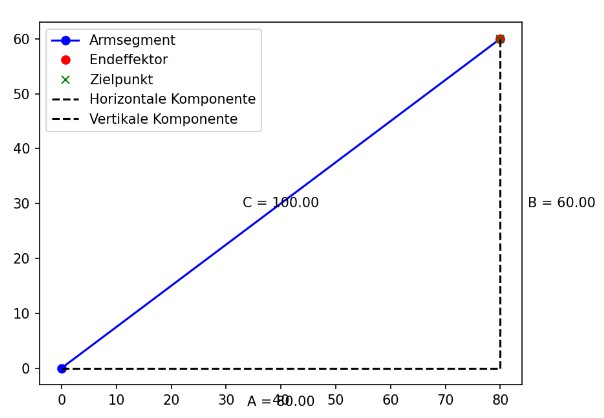
\includegraphics[width = \linewidth]{Bild 1}
        \caption{Berechnung Distanz}
    \end{figure}

    \lstinputlisting[language=Python, firstline=59, lastline=60, caption={Neuberechnung der Winkel beim Drag}]{PuzzleSpiel.py}

    Für die Berechnung bei 1, 2 und 3 Gelenken ist unterschiedlicher Code erforderlich. Dieser wird je
    nach Bedarf durch eine if-else-Anweisung aufgerufen.

    \subsubsubsection{Berechnung für 1 Gelenk}
    Handelt es sich um nur ein Gelenk, soll der Endeffektor des Arms in Richtung des Zielpunkts
    bewegt werden. Für die genauen Koordinaten wird die zuvor berechnete Distanz und der Winkel des
    Armsegments benötigt. Diesen erhält man durch Einsetzen der Koordinaten in die
    Arcustangens-Funktion.

    \[
        \theta=arctan(\frac{B}{A})
    \]
    \[
        \theta=arctan(\frac{60}{80})=0,64 (36,87^\circ)
    \]

    \begin{figure}[h]
        \centering
        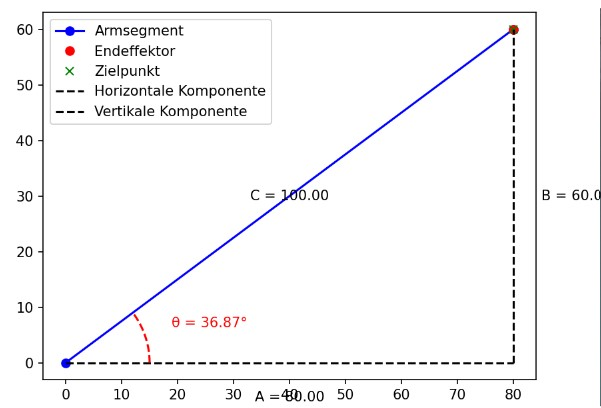
\includegraphics[width = \linewidth]{Bild 2}
        \caption{Berechnung Schulterwinkel für 1 Armsegment}
    \end{figure}

    \lstinputlisting[language=Python, firstline=63, lastline=65, caption={Winkelberechnung für ein Gelenk}]{PuzzleSpiel.py}

    Multipliziert man nun die Armlänge mit dem Sinus beziehungsweise dem Kosinus des Winkels, erhält
    man den Endeffektor.

    \[
        x=c * cos(\theta)
    \]
    \[
        y=c * sin(\theta)
    \]
    \[
        x=100 * cos(0,64)=80
    \]
    \[
        y=100 * sin(0,64)=60
    \]

    \lstinputlisting[language=Python, firstline=93, lastline=95, caption={Berechnung des Endeffektors für ein Gelenk beim Drag}]{PuzzleSpiel.py}


    \subsubsubsection{Berechnung für 2 Gelenke}
    Bei der Berechnung der Winkel mit zwei Armsegmenten wird wie bei einem Armsegment auch zuerst
    die Distanz zwischen dem Endeffektor und dem Ursprung berechnet. Zusätzlich sind die Längen der
    beiden Armsegmente gegeben, woraus ein Dreieck mit drei bekannten Seitenlängen entsteht.

    \begin{figure}[h]
        \centering
        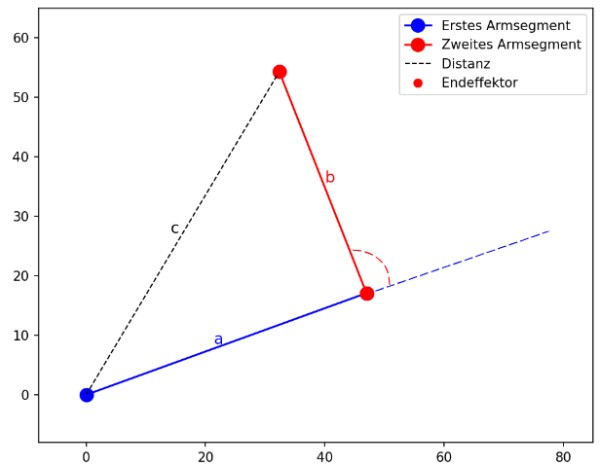
\includegraphics[width = \linewidth]{Bild 3}
        \caption{Berechnung Ellenbogenwinkel für 2 Armsegmente}
    \end{figure}

    \[
        a=50
    \]
    \[
        b=40
    \]
    \[
        c=63,25
    \]

    Für die Berechnung des Ellenbogenwinkels kann nun der Kosinussatz umgestellt nach dem Winkel
    angewendet werden.

    \[
        cos(\theta)= \frac{a^2+b^2-c^2}{2*a*b}
    \]
    \[
        cos(\theta)= \frac{50^2+40^2-63,25^2}{2*20*40}
    \]
    \[
        \theta= arccos(0,025) = 89,86^\circ
    \]

    Nachdem der Ellenbogenwinkel berechnet wurde, kann mit dessen Hilfe auch der Schulterwinkel
    berechnet werden, indem folgende Formel verwendet wird.

    \[
        \alpha = arctan(\frac{y}{x}) - arctan(\frac{b*cos(\theta)}{a+b*sin(\theta)})
    \]
    \[
        \alpha = arctan(\frac{20}{60}) - arctan(\frac{40*cos(89,86^\circ)}{50+40*sin(89,86^\circ)})                    \]
    \[
        \alpha = 18,43^\circ - 37,97^\circ = -19,55^\circ
    \]

    \lstinputlisting[language=Python, firstline=68, lastline=73, caption={Winkelberechnungen für zwei Gelenke}]{PuzzleSpiel.py}

    Nachdem beide Winkel berechnet wurden, kann mit Hilfe der Armlängen der Arm konstruiert werden.
    Die Positionen des Ellenbogengelenks und des Endeffektors werden durch Einsetzen der Winkel in
    Sinus- und Kosinusfunktionen multipliziert mit der Armlänge bestimmt.

    Ellenbogengelenk:

    \[
        x1 = a * cos(\theta)
    \]
    \[
        y1 = a * sin(\theta)
    \]

    \[
        x1 = 50 * cos(-19,55^\circ) = 47,12
    \]
    \[
        y1 = 50 * sin(.19,55^\circ) = 16,73
    \]

    Endeffektor:

    \[
        x2 = x1 + b * cos(\theta + \alpha)
    \]
    \[
        y2 = y1 + b * sin(\theta + \alpha)
    \]

    \[
        x2 = 47,12 + 40 * cos(-19,55^\circ + 89,86^\circ) = 60,6
    \]
    \[
        y2 = 16,73 + 40 * sin(-19,55^\circ + 89,86^\circ) = 54,4
    \]

    Diese Punkte werden miteinander verbunden und werden dauerhaft aktualisiert, wodurch der
    Roboterarm dargestellt wird und sich den Bewegungen anpasst.

    \lstinputlisting[language=Python, firstline=96, lastline=98, caption={Berechnung des Endeffektors für zwei Gelenke beim Drag}]{PuzzleSpiel.py}

    \subsubsubsection{Berechnung für 3 Gelenke}
    Die Winkel für die 3 Gelenke werden die Formeln genutzt, die man durch die gegebenen Werte aufstellen kann,
    um die fehlenden Winkel rauszubekommen. Das geschieht durch ein numerisches Optimierungsverfahren, das darauf
    abzielt, die Differenzen zwischen den berechneten Werten und den zuvor gegebenen Winkeln zu minimieren.
    Die beiden Formeln werden aus der folgenden Skizze ersichtlich:

    \begin{figure}[h]
        \centering
        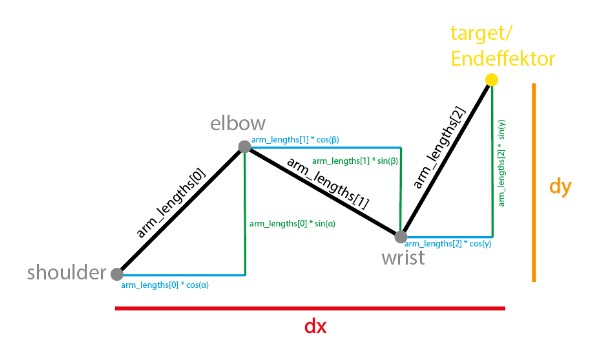
\includegraphics[width = \linewidth]{Bild 5}
        \caption{Bestimmung Endeffektor für 3 Armsegmente}
    \end{figure}

    \[
        dx = armlengths[0] * cos(\alpha) + armlengths[1] * cos(\beta) + armlength[2] * cos(\gamma)
    \]
    \[
        dx = armlengths[0] * sin(\alpha) + armlengths[1] * sin(\beta) + armlength[2] * sin(\gamma)
    \]

    \lstinputlisting[language=Python, firstline=83, lastline=89, caption={Berechnung der Positions-Differenzen}]{PuzzleSpiel.py}

    \begin{figure}[h]
        \centering
        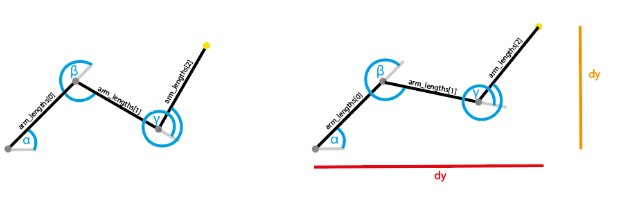
\includegraphics[width = \linewidth]{Bild 6}
        \caption{Winkelberechnung bei 3 Armsegmenten}
    \end{figure}

    In dem Beispiel ist die Ausgangsposition vom Roboterarm auf der linken Skizze abgebildet und die
    Winkel und Armlängen sind:

    \[
        \alpha = 0,5*\pi
    \]
    \[
        \beta = 1,5 * \pi
    \]
    \[
        \gamma = 2,5 * \pi
    \]

    \[
        armlengths[0] = 100
    \]
    \[
        armlengths[1] = 105
    \]
    \[
        armlengths[2] = 110
    \]

    \[
        dx = 250
    \]
    \[
        dy = 150
    \]

    Diese Werte werden zum Initial Guess, das sind die Winkel, an denen sich der Algorithmus
    orientiert.

    \lstinputlisting[language=Python, firstline=77, lastline=77, caption={Initial Guess}]{PuzzleSpiel.py}

    Die Formeln sähen mit den gegebenen Werten folgendermaßen aus:

    \[
        0 = 100 * cos(\alpha) + 105 * cos(\beta) + 110 * cos(\gamma) -250
    \]
    \[
        0 = 100 * sin(\alpha) + 105 * sin(\beta) + 110 * sin(\gamma) -150
    \]

    Nun wird mit den obigen aufgestellten Formeln und den Orientierungswerten der least squares-
    Algorithmus aufgerufen. In dem Ergebnis sind dann die optimalen Winkel für den Roboterarm.

    \lstinputlisting[language=Python, firstline=78, lastline=79, caption={Berechnung des optimalsten Winkel}]{PuzzleSpiel.py}

    Das Ergebnis der Rechnung lautet somit:
    \[
        self.shoulderangle = 0,27 *\pi
    \]
    \[
        self.elbowangle = 1,72 *\pi
    \]
    \[
        self.wristangle = 2,25 *\pi
    \]

    Schließlich müssen auch noch die Positionen aller Gelenke und des Endeffektors berechnet werden.
    Die Position der Schulter, welche sich beim Bewegen des Roboterarmes nicht mitbewegt, liegt bei
    [200, 200].

    \[
        elbow = [200, 200] + [100 * cos(0,27 * \pi), 100 * sin(0,27*\pi)] = [266, 275]
    \]
    \[
        wrist = [266, 275] + [105 * cos(0,27 * \pi + 1,72 * \pi), 105 * sin(0,27*\pi + 1,72 * \pi)] = [371, 272]
    \]
    \[
        endeffector = [371, 272] + [ 110 * cos(0,27*\pi + 1,72*\pi + 2,25*\pi),
    \]
    \[
        110 * sin(0,27*\pi + 1,72*\pi + 2,25*\pi)] = [451, 347]
    \]

    \lstinputlisting[language=Python, firstline=100, lastline=103, caption={Berechnung aller Positionen}]{PuzzleSpiel.py}

    \subsection{GUI-Klasse}
    Die GUI-Klasse initialisiert die Hauptkomponenten der Benutzeroberfläche. Sie erstellt ein Canvas-Widget,
    auf dem der Roboterarm und die Puzzleteile angezeigt werden, sowie verschiedene Konfigurationsoptionen für
    die Steuerung des Roboterarms.

    \subsubsection{Konfigurationspanel}
    Das Konfigurationspanel ermöglicht es dem Benutzer, die Anzahl der Gelenke sowie die Längen der Arme
    des Roboterarms anzupassen. Diese Einstellungen werden dabei dynamisch aktualisiert, sodass Änderungen
    in Echtzeit umgesetzt und visuell dargestellt werden.

    \lstinputlisting[language=Python, firstline=137, lastline=164, caption={Panel für das Konfigurationsmenü}]{PuzzleSpiel.py}

    Die Methoden \textit{update\_num\_joints()}, \textit{update\_arm\_length1()},
    \textit{update\_arm\_length2()} und
    \textit{update\_arm\_length3()} dienen dazu, die Parameter des Roboterarms zu aktualisieren und ihn
    anschließend neu zu zeichnen.
    Die Methode \textit{update\_num\_joints()} aktualisiert die Anpassungsmöglichkeiten des Roboterarms. Je nach
    der gewählten Anzahl der Gelenke werden die entsprechenden Konfigurationsoptionen des Roboterarms
    angezeigt oder ausgeblendet. Nach der Aktualisierung wird der Roboterarm neu gezeichnet, um die
    Änderungen visuell darzustellen.

    \lstinputlisting[language=Python, firstline=166, lastline=198, caption={Aktualisieren der Parameter des Roboterarms}]{PuzzleSpiel.py}

    \subsubsection{Puzzleteile und Grid (Zielfläche)}
    Die Puzzleteile werden erstellt und zufällig auf dem Canvas platziert. Ein 2x2-Grid dient als
    Zielbereich für die Puzzleteile. Ein Bild ist hinterlegt, aus welchem die Puzzleteile erstellt werden.
    Das Bild ist flexibel austauschbar, solange der Dateiname gleich bezeichnet und im gleichen Verzeichnis wie die
    Spiel-Datei gelegt wird. Vorerst bildet ein 2x2-Grid bestehend aus Quadraten das Zielfeld, in welches die Puzzleteile
    hineingelegt werden sollen. Auf dieser Basis wird das Bild auf die benötigte Größe skaliert, sodass
    das Zielfeld vom Bild abgedeckt wird. Anschließend werden die Puzzleteile mit der vorher definierten
    Feldgröße erstellt, indem entsprechend große Teile aus dem Bild ausgeschnitten werden. Jedes
    Puzzleteil wird mit einem Eventlistener verbunden und in eine Liste von Puzzleteilen hinzugefügt.

    \lstinputlisting[language=Python, firstline=200, lastline=217, caption={Erstellung der Puzzleteile}]{PuzzleSpiel.py}


    Das Grid wird auf ähnliche Weise erstellt wie die Puzzleteile. Hierbei werden Quadrate in der zuvor
    definierten Feldgröße ohne Lücken aneinandergesetzt. Abschließend wird jedem Quadrat eine Position
    zugewiesen.

    \lstinputlisting[language=Python, firstline=219, lastline=229, caption={Erstellung des Grids}]{PuzzleSpiel.py}

    \subsubsection{Puzzleteile bewegen}
    Um den Roboterarm zu bewegen, muss dieser mit einem Linksklick ausgewählt werden. Dabei wird zunächst
    überprüft, ob sich der Abstand zwischen dem Mauszeiger und dem Endeffektor innerhalb eines Radius
    von 10 befindet.

    \lstinputlisting[language=Python, firstline=237, lastline=240, caption={Linksklick auf den Endeffektor}]{PuzzleSpiel.py}
    \lstinputlisting[language=Python, firstline=277, lastline=280, caption={Feld-Definition in dem der Endeffektor ausgewählt werden kann}]{PuzzleSpiel.py}

    Während der Bewegung des Arms wird die Methode \textit{on\_drag()} kontinuierlich ausgeführt. In diesem
    Prozess werden fortlaufend die Position des Endeffektors sowie die des ausgewählten Puzzleteils an
    die Position des Mauszeigers angepasst.

    \newpage

    \lstinputlisting[language=Python, firstline=242, lastline=251, caption={Fortlaufende Anpassung der Endeffektor Position}]{PuzzleSpiel.py}

    \subsubsection{Puzzleteile aufnehmen und ablegen}
    Durch einen Rechtsklick soll der Endeffektor ein Puzzleteil „greifen“ können. Falls der Greifarm noch
    kein Puzzleteil aufgenommen hat, wird ihm das Puzzleteil zugewiesen, dessen Koordinaten mit der
    Position des Endeffektors übereinstimmen. Danach wird der Endeffektor zentriert auf das Puzzleteil
    positioniert.

    Wenn der Greifarm bereits ein Puzzleteil aufgenommen hat, werden die Koordinaten des Puzzleteils mit
    den Koordinaten der Quadrate im Zielfeld verglichen. Ein Puzzleteil wird auf einem Quadrat platziert,
    wenn der Abstand zwischen den Koordinaten kleiner als 3 ist. Diese Bedingung wird durch den logischen
    Ausdruck in der Methode \textit{is\_inside()} überprüft. Ist dies zutreffend, wird das Puzzleteil auf das
    entsprechende Quadrat im Grid gesetzt. Diese Vorgehensweise trägt zur Verbesserung der
    Benutzerfreundlichkeit bei.

    \lstinputlisting[language=Python, firstline=257, lastline=275, caption={Aufnehmen und ablegen von Puzzleteilen}]{PuzzleSpiel.py}
    \lstinputlisting[language=Python, firstline=323, lastline=333, caption={Überprüfung, ob das Puzzleteil mit einer Toleranz im Grid liegt}]{PuzzleSpiel.py}

    \subsubsection{Überprüfung der Position}
    Die Überprüfung beginnt erst nach Betätigung des Knopfes „Check Positions“. Bei diesem Schritt
    werden die hinterlegten Positionen der Puzzleteile mit den aktuellen Positionen verglichen, um
    sicherzustellen, dass alle Teile korrekt platziert sind. Ein Zähler wird nur dann erhöht, wenn die
    Positionen der Puzzleteile mit den vorgegebenen Positionen übereinstimmen. Dieser Zähler gibt nach
    der Überprüfung an, wie viele Puzzleteile korrekt positioniert wurden.

    \lstinputlisting[language=Python, firstline=308, lastline=321, caption={Überprüfung der Position}]{PuzzleSpiel.py}

    \subsection{Kollisionserkennung}
    Diese Mechanismen tragen dazu bei, eine präzise und benutzerfreundliche Interaktion mit dem
    Roboterarm und den Puzzleteilen zu gewährleisten. Die Kollisionserkennung ist entscheidend für
    die korrekte Funktionalität der Anwendung und die Genauigkeit der Interaktionen.

    \subsubsection{Kollisionserkennung beim Drag \& Drop von Puzzleteilen}
    Ein zentraler Aspekt der Kollisionserkennung betrifft das Drag & Drop von Puzzleteilen. Hierbei wird
    die Methode \textit{on\_right\_click(self, event)} verwendet, um den Greifarm Puzzleteile mit der rechten
    Maustaste aufnehmen oder ablegen zu lassen. Um sicherzustellen, dass das Puzzleteil korrekt auf
    einem Quadrat positioniert wird, wird die Methode \textit{is\_inside(self, square\_coords, piece\_coords)}
    verwendet. Diese Methode überprüft, ob die Randkoordinaten des Puzzleteils innerhalb der Grenzen
    eines Grid-Quadrats liegen, wobei eine Toleranz von 3 berücksichtigt wird. Diese Toleranz hilft,
    kleine Abweichungen in der Positionierung auszugleichen und gewährleistet eine präzise Platzierung
    der Puzzleteile, was zu einer höheren Benutzerfreundlichkeit beiträgt.

    \subsubsection{Kollisionserkennung bei der Positionierung des Endeffektors}
    Zusätzlich zur Platzierung von Puzzleteilen ist die Kollisionserkennung auch bei der Positionierung
    des Endeffektors von Bedeutung. Die Methode \textit{on\_press(self, event)} wird aktiviert, wenn der Benutzer
    die Maus in der Nähe des Endeffektors klickt, um den Drag-Modus zu starten. Um festzustellen, ob sich
    der Mauszeiger in der Nähe des Endeffektors befindet, verwendet die Methode
    \textit{is\_near\_end\_effector(self, x, y)} die euklidische Distanz zwischen der Position des Mauszeigers und
    der Position des Endeffektors. Ein Radius von 10 wird hierbei als Kriterium verwendet, um die Nähe
    zu überprüfen.

    \subsubsection{Kollisionserkennung während der Armbewegung}
    Während der Armbewegung wird die Methode \textit{on\_drag(self, event)} aufgerufen, die es ermöglicht, dass
    das ausgewählte Puzzleteil der Bewegung des Roboterarms folgt. Hierbei wird sichergestellt, dass das
    Puzzleteil immer entsprechend der Position des Endeffektors aktualisiert wird.


    \section{Erweiterungsmöglichkeiten}
    Das Projekt bietet mehrere Ansatzpunkte für zukünftige Erweiterungen. Eine wesentliche Möglichkeit besteht in
    der Erweiterung der Konfigurationsmöglichkeiten des Roboterarms. Derzeit können Benutzer grundlegende Parameter
    anpassen, um die Kinematik des Arms zu erforschen. Weitere Entwicklungen könnten es ermöglichen, die
    Konfiguration des Roboterarms noch detaillierter vorzunehmen. Dazu könnten erweiterte Optionen zur
    Feinabstimmung der Gelenkwinkel und zur Anpassung der Geschwindigkeiten gehören sowie zusätzliche
    Konfigurationsparameter, die eine noch präzisere Anpassung und Untersuchung der Bewegungsabläufe ermöglichen.

    Neben den funktionalen Erweiterungen besteht auch die Möglichkeit zur Verbesserung des Designs der
    Benutzeroberfläche. Die aktuelle Benutzeroberfläche bietet eine funktionale Grundstruktur, jedoch besteht
    Potenzial für eine ansprechendere und intuitivere Gestaltung. Eine Überarbeitung könnte detailreiche Grafiken
    und eine Anleitung zur Interaktiven Nutzung, beinhalten. Die Benutzerfreundlichkeit würde durch diese
    Änderungen deutlich verbessert werden, denn sie ermöglichen eine klarere und intuitivere Navigation
    durch die Simulation.


    \section{Schlussfolgerung}
    Das entwickelte 2D-Puzzle-Spiel mit Roboterarm Steuerung bietet eine Grundlage für die interaktive Simulation
    der Roboterkinematik. Durch die Möglichkeit, verschiedene Konfigurationen des Roboterarms zu testen, können
    Benutzer ein tieferes Verständnis für die Funktionsweise und Bewegungsabläufe von Roboterarmen entwickeln.
    Dabei haben sich die flexible Konfigurationsmöglichkeit und die Drag-and-Drop-Funktionalität als zentrale
    Merkmale der Anwendung herausgestellt.

    Während der Umsetzung des Projekts haben wir wertvolle Erkenntnisse gewonnen. Besonders hervorzuheben ist,
    dass die Implementierung eines Roboterarms mit drei Gelenken deutlich komplexer und fehleranfälliger war als
    ursprünglich erwartet. Die Herausforderungen bei der mathematischen Modellierung und der kinematischen Steuerung
    haben gezeigt, wie anspruchsvoll die Entwicklung eines solchen Systems sein kann. Insbesondere bei der exakten
    Positionierung der Endeffektoren, traten immer wieder Schwierigkeiten auf. Es benötigte mehrere Anläufe und
    unterschiedliche Herangehensweisen, um die präzise Berechnung der Gelenkwinkel und deren Koordination erfolgreich
    umzusetzen. Der Prozess umfasste einige Anpassungen und häufige Fehlersuche, doch zum Schluss gelang die genaue
    Positionierung des Endeffektors.

    Trotz der sorgfältigen Planung und Implementierung sind weiterhin Verbesserungen und Erweiterungen möglich,
    um die Funktionalität und Benutzerfreundlichkeit weiter zu optimieren. Die gesammelten Erfahrungen haben unsere
    Kenntnisse in der Roboterkinematik und der praktischen Anwendung von Simulationstechniken erheblich erweitert.

    \newpage

    \begin{thebibliography}{20} % Breite für die Nummern
        \bibitem{Far01}
        Julia Dubcova: {\it Steuerung eines 5-DOF-Handhabungsroboters in Arbeitsraumkoordinaten} \\
        URL: https://reposit.haw-hamburg.de/handle/20.500.12738/5263 \\
        (Stand: 24.07.2024 15:30 Uhr)
        \bibitem{Far02}
        Prof. Dr.-Ing. Oliver Tessmann et al.: {\it Tactile Robotic Assembly} \\
        URL:
        \raggedright https://www.bbsr.bund.de/BBSR/DE/veroeffentlichungen/bbsr-online/2024/bbsr-online-05-2024-dl.pdf \\
        (Stand: 24.07.2024 15:25 Uhr)
        \bibitem{Far03}
        Rick Parent, {\it Computer Animation: Algorithms and Techniques} \\
        2. Auflage, Morgan Kaufmann, ISBN 9780124158429
    \end{thebibliography}

\end{document}